% !Mode:: "TeX:UTF-8"

\BiChapter{基于词典与知识库的方法}{}
\label{c:dict lib}
词典或知识库是一种描述词语语义的语言学资料。这里的词典并不像我们常用的词典那样使用自然语言解释词语,它会将词语组织成一定的结构,并且使用形式化的方式进行描述。这就为词语的语义提供了一种计算机容易理解的表示形式。

在英文方面,最著名的词典或知识库是普林斯顿大学开发的WordNet\citeup{Miller1995}。而在中文方面,则有董振东教授开发的知网(HowNet)与梅家驹等人开发的同义词词林。后者经过了哈尔滨工业大学信息检索实验室的改进,形成了同义词词林扩展版。

本课题将会给出一种基于同义词词林扩展版的词语相似度计算方法。这种方法并不能独立工作,而是需要与第\ref{c:ensemble}章介绍的方法相配合以产生最终的结果。

\BiSection{同义词词林扩展版介绍}{}
最初版本的同义词词林包含53859个词条,其中,有14706个词条由于现代的使用频率过低,成为了罕用词与非常用词。同义词词林扩展版删除了这些词语,并且增补完善了一定数量的词语,使得最终的词条数量达到了77343条。

在结构上,同义词词林扩展版将词条分类组织为一个树状结构,如图\ref{f:cilin layers}所示。分类的层次共有5层,随着层次的增加,词语语义的划分越来越细。第五层的词类称为原子词群。一个原子词群中的词语可能是同义词,可能是互相相关的非同义词,也可能一个原子词群中仅有一个词语。同一个词语可能同时出现在多个不同的原子词群中。这意味着这个词语是一个多义词。原子词群的编码方式如表\ref{t:cilin code}所示,其中,“=”表示一个原子词群是同义词,而“\#”表示一个原子词群是同类词语,“@”表示原子词群内只有一个词语。

\begin{figure}[h]
	\centering
	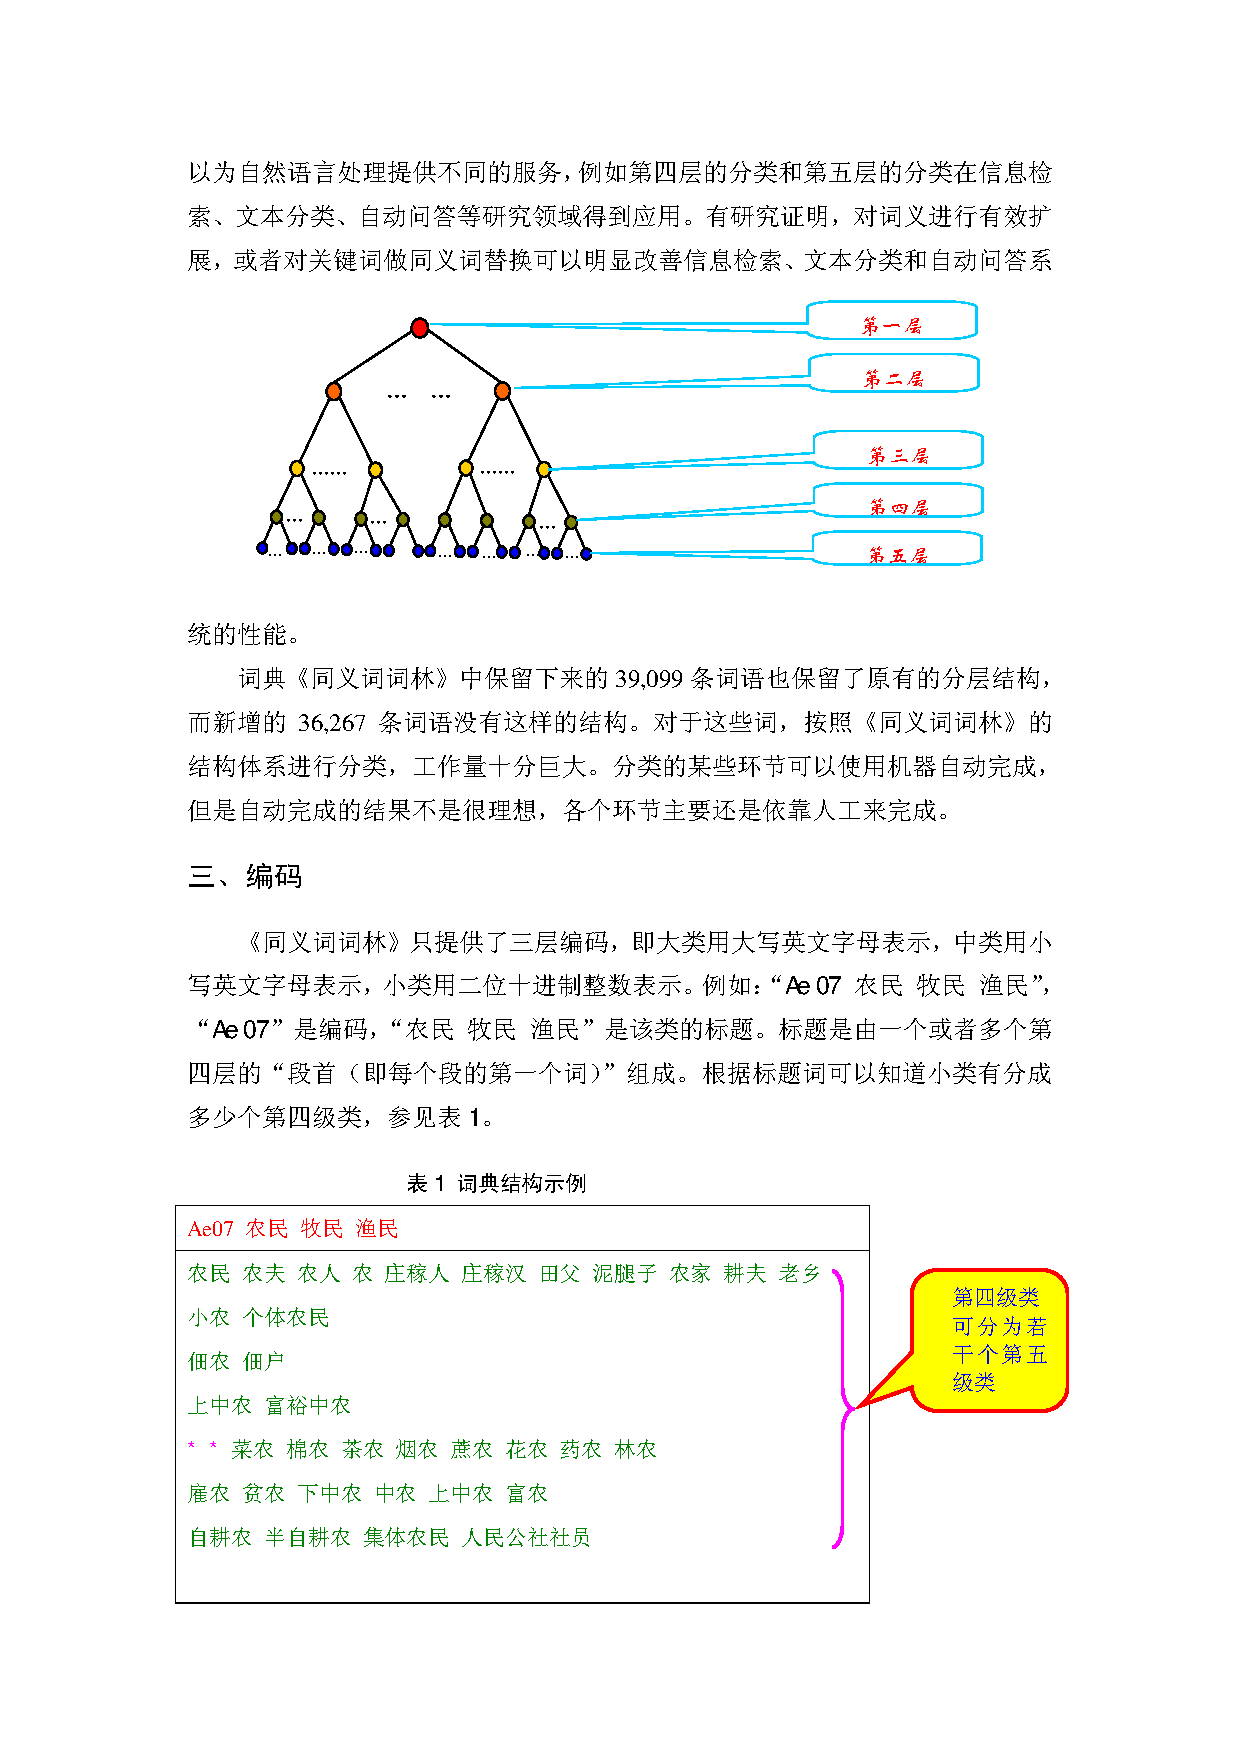
\includegraphics[trim={4.3cm 20.1cm 4.3cm 5.05cm},clip]{Cilin-layers}
	\caption{同义词词林扩展版的结构(来自同义词词林扩展版说明)}
	\label{f:cilin layers}
	\vspace{-1em}
\end{figure}

\begin{table}[h]
	\caption{原子词群的编码方式(来自同义词词林扩展版说明)}
	\label{t:cilin code}
	\vspace{0.5em}
	\centering
	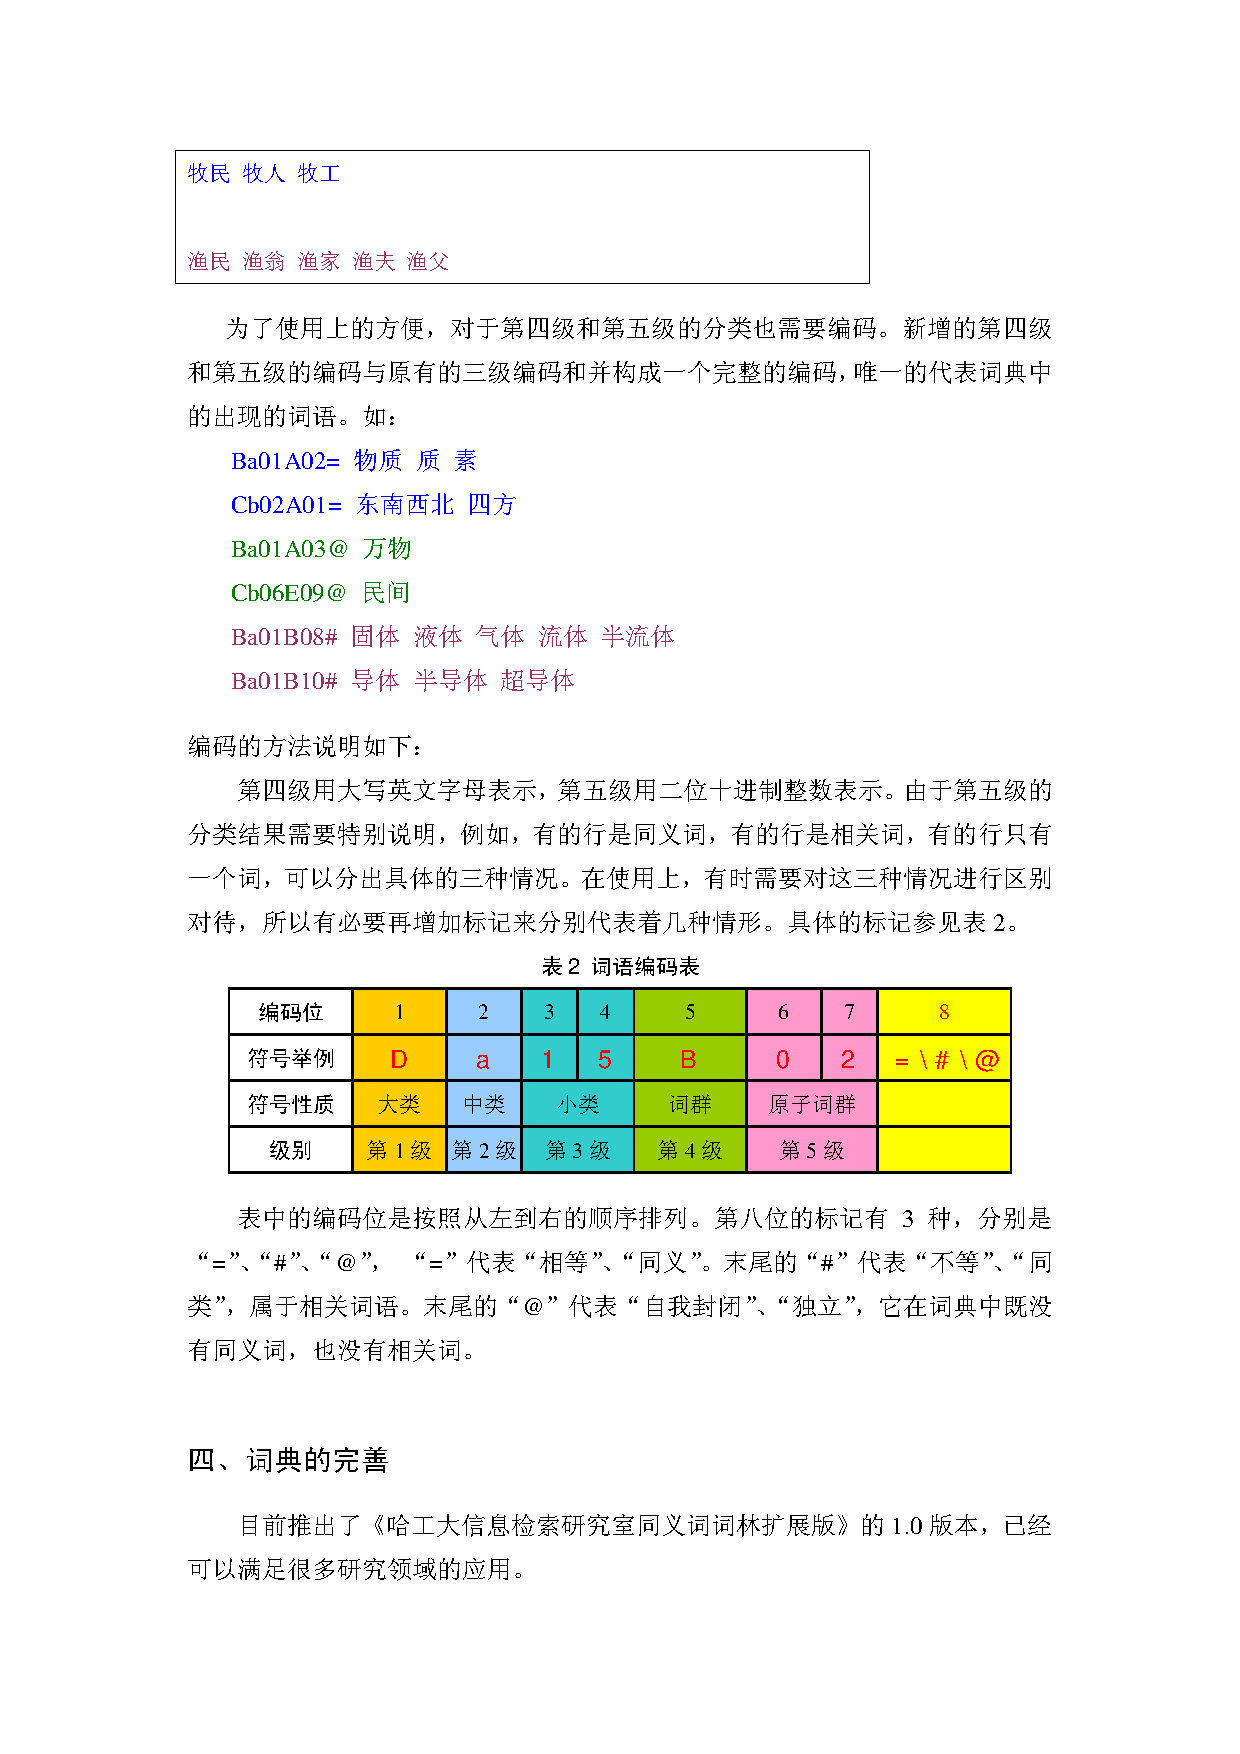
\includegraphics[trim={3.85cm 9.83cm 3.85cm 16.73cm},clip]{Cilin-code}
\end{table}

\BiSection{特征提取}{}
\label{s:dict features}
传统的基于词典与知识库的词语相似度计算方法都是从词典与知识库中提取与目标词语对有关的一些特征,并使用一些公式组合特征以得到结果。本方法也使用类似的方法,从同义词词林扩展版中提取出一些向量特征。

对于每一个词语对,本方法提取的特征是一个三维向量$(d, s_1, s_2)$。我们先设$d'$为同时包含两个词语的最深的类别的深度(也就是最近公共祖先),如果有词语同时属于多个原子词群,则选$d'$值最大的。当两个词语不属于相同的一级类别时,$d' = 0$。对于$d' < 5$的情况,$d = d'$,而当$d' = 5$(也就是说,两个词语属于同一个原子词群)时,需要分情况讨论。当原子词群是同义词时,$d = d' + 1$,否则$d = d'$。$s_1$与$s_2$分别是包含每个词语的原子类群数量(每个词语的词义个数)。

与传统方法不同的是,本方法并不根据提取的特征直接计算词语相似度,而是将特征直接作为模型的输出。其原因将在第\ref{s:ensemble features}小节说明。